\documentclass{standalone}
\usepackage{tikz}
\usetikzlibrary{patterns, positioning}


\begin{document}
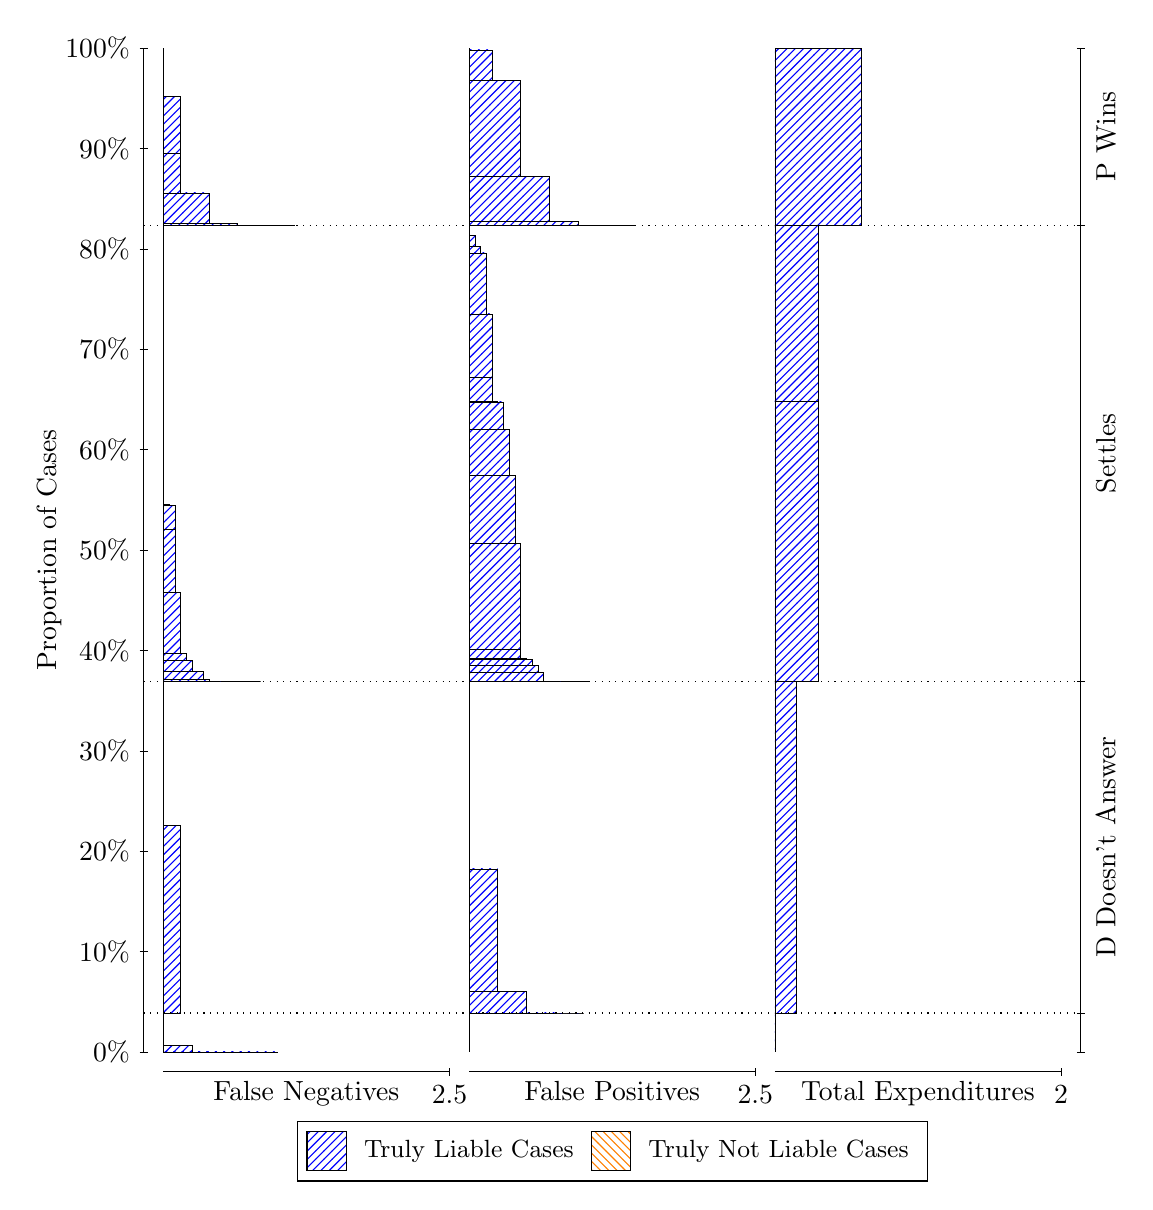
\begin{tikzpicture}
\draw[black, very thin] (1.5,1.75) -- (1.5,14.5);
\node[rotate=90, text=black, anchor=center] at (0.3, 8.125) {Proportion of Cases};
\draw[black, very thin] (1.45,1.75) -- (1.55,1.75);
\node[text=black, anchor=east] at (1.45, 1.75) {0\%};
\draw[black, very thin] (1.45,3.025) -- (1.55,3.025);
\node[text=black, anchor=east] at (1.45, 3.025) {10\%};
\draw[black, very thin] (1.45,4.3) -- (1.55,4.3);
\node[text=black, anchor=east] at (1.45, 4.3) {20\%};
\draw[black, very thin] (1.45,5.575) -- (1.55,5.575);
\node[text=black, anchor=east] at (1.45, 5.575) {30\%};
\draw[black, very thin] (1.45,6.85) -- (1.55,6.85);
\node[text=black, anchor=east] at (1.45, 6.85) {40\%};
\draw[black, very thin] (1.45,8.125) -- (1.55,8.125);
\node[text=black, anchor=east] at (1.45, 8.125) {50\%};
\draw[black, very thin] (1.45,9.4) -- (1.55,9.4);
\node[text=black, anchor=east] at (1.45, 9.4) {60\%};
\draw[black, very thin] (1.45,10.675) -- (1.55,10.675);
\node[text=black, anchor=east] at (1.45, 10.675) {70\%};
\draw[black, very thin] (1.45,11.95) -- (1.55,11.95);
\node[text=black, anchor=east] at (1.45, 11.95) {80\%};
\draw[black, very thin] (1.45,13.225) -- (1.55,13.225);
\node[text=black, anchor=east] at (1.45, 13.225) {90\%};
\draw[black, very thin] (1.45,14.5) -- (1.55,14.5);
\node[text=black, anchor=east] at (1.45, 14.5) {100\%};

\draw[black, very thin] (13.4,1.75) -- (13.4,14.5);
\draw[black, very thin] (13.35,1.75) -- (13.45,1.75);
\node[anchor=west] at (13.35, 1.75) {};
\draw[black, very thin] (13.35,2.2449) -- (13.45,2.2449);
\node[anchor=west] at (13.35, 2.2449) {};
\draw[black, very thin] (13.35,6.459) -- (13.45,6.459);
\node[anchor=west] at (13.35, 6.459) {};
\draw[black, very thin] (13.35,12.251) -- (13.45,12.251);
\node[anchor=west] at (13.35, 12.251) {};
\draw[black, very thin] (13.35,14.5) -- (13.45,14.5);
\node[anchor=west] at (13.35, 14.5) {};

\draw[black, very thin, pattern color=blue, pattern=north east lines] (1.75,1.75) rectangle (3.2033,1.75);
\draw[black, very thin, pattern color=blue, pattern=north east lines] (1.75,1.75) rectangle (2.84,1.75);
\draw[black, very thin, pattern color=blue, pattern=north east lines] (1.75,1.75) rectangle (2.4767,1.7507);
\draw[black, very thin, pattern color=blue, pattern=north east lines] (1.75,1.7507) rectangle (2.1133,1.831);
\draw[black, very thin, pattern color=orange, pattern=north west lines] (1.75,1.831) rectangle (1.75,1.831);
\draw[black, very thin, pattern color=blue, pattern=north east lines] (1.75,1.831) rectangle (1.75,2.2449);
\draw[black, very thin, pattern color=blue, pattern=north east lines] (1.75,2.2449) rectangle (1.968,4.63);
\draw[black, very thin, pattern color=orange, pattern=north west lines] (1.75,4.63) rectangle (1.75,4.63);
\draw[black, very thin, pattern color=blue, pattern=north east lines] (1.75,4.63) rectangle (1.75,6.459);
\draw[black, very thin, pattern color=blue, pattern=north east lines] (1.75,6.459) rectangle (2.9853,6.459);
\draw[black, very thin, pattern color=blue, pattern=north east lines] (1.75,6.459) rectangle (2.84,6.459);
\draw[black, very thin, pattern color=blue, pattern=north east lines] (1.75,6.459) rectangle (2.6947,6.459);
\draw[black, very thin, pattern color=blue, pattern=north east lines] (1.75,6.459) rectangle (2.622,6.4591);
\draw[black, very thin, pattern color=blue, pattern=north east lines] (1.75,6.4591) rectangle (2.5493,6.4591);
\draw[black, very thin, pattern color=blue, pattern=north east lines] (1.75,6.4591) rectangle (2.4767,6.4591);
\draw[black, very thin, pattern color=blue, pattern=north east lines] (1.75,6.4591) rectangle (2.404,6.4592);
\draw[black, very thin, pattern color=blue, pattern=north east lines] (1.75,6.4592) rectangle (2.3313,6.4851);
\draw[black, very thin, pattern color=blue, pattern=north east lines] (1.75,6.4851) rectangle (2.2587,6.5821);
\draw[black, very thin, pattern color=blue, pattern=north east lines] (1.75,6.5821) rectangle (2.186,6.5825);
\draw[black, very thin, pattern color=blue, pattern=north east lines] (1.75,6.5825) rectangle (2.1133,6.7277);
\draw[black, very thin, pattern color=blue, pattern=north east lines] (1.75,6.7277) rectangle (2.0407,6.811);
\draw[black, very thin, pattern color=blue, pattern=north east lines] (1.75,6.811) rectangle (1.968,7.5865);
\draw[black, very thin, pattern color=blue, pattern=north east lines] (1.75,7.5865) rectangle (1.8953,8.3884);
\draw[black, very thin, pattern color=blue, pattern=north east lines] (1.75,8.3884) rectangle (1.8953,8.693);
\draw[black, very thin, pattern color=blue, pattern=north east lines] (1.75,8.693) rectangle (1.8227,8.7037);
\draw[black, very thin, pattern color=orange, pattern=north west lines] (1.75,8.7037) rectangle (1.75,8.7037);
\draw[black, very thin, pattern color=blue, pattern=north east lines] (1.75,8.7037) rectangle (1.75,12.251);
\draw[black, very thin, pattern color=blue, pattern=north east lines] (1.75,12.251) rectangle (3.4213,12.251);
\draw[black, very thin, pattern color=blue, pattern=north east lines] (1.75,12.251) rectangle (3.058,12.251);
\draw[black, very thin, pattern color=blue, pattern=north east lines] (1.75,12.251) rectangle (2.6947,12.274);
\draw[black, very thin, pattern color=blue, pattern=north east lines] (1.75,12.274) rectangle (2.3313,12.66);
\draw[black, very thin, pattern color=blue, pattern=north east lines] (1.75,12.66) rectangle (1.968,13.16);
\draw[black, very thin, pattern color=blue, pattern=north east lines] (1.75,13.16) rectangle (1.968,13.884);
\draw[black, very thin, pattern color=orange, pattern=north west lines] (1.75,13.884) rectangle (1.75,13.884);
\draw[black, very thin, pattern color=blue, pattern=north east lines] (1.75,13.884) rectangle (1.75,14.5);
\draw[black, very thin, pattern color=orange, pattern=north west lines] (5.6333,1.75) rectangle (5.6333,1.75);
\draw[black, very thin, pattern color=blue, pattern=north east lines] (5.6333,1.75) rectangle (5.6333,2.2449);
\draw[black, very thin, pattern color=orange, pattern=north west lines] (5.6333,2.2449) rectangle (7.0867,2.2449);
\draw[black, very thin, pattern color=blue, pattern=north east lines] (5.6333,2.2449) rectangle (7.0867,2.2449);
\draw[black, very thin, pattern color=blue, pattern=north east lines] (5.6333,2.2449) rectangle (6.7233,2.2471);
\draw[black, very thin, pattern color=blue, pattern=north east lines] (5.6333,2.2471) rectangle (6.36,2.5165);
\draw[black, very thin, pattern color=blue, pattern=north east lines] (5.6333,2.5165) rectangle (5.9967,4.0738);
\draw[black, very thin, pattern color=blue, pattern=north east lines] (5.6333,4.0738) rectangle (5.6333,6.459);
\draw[black, very thin, pattern color=orange, pattern=north west lines] (5.6333,6.459) rectangle (7.1593,6.459);
\draw[black, very thin, pattern color=blue, pattern=north east lines] (5.6333,6.459) rectangle (7.1593,6.459);
\draw[black, very thin, pattern color=orange, pattern=north west lines] (5.6333,6.459) rectangle (7.014,6.459);
\draw[black, very thin, pattern color=blue, pattern=north east lines] (5.6333,6.459) rectangle (7.014,6.459);
\draw[black, very thin, pattern color=orange, pattern=north west lines] (5.6333,6.459) rectangle (6.8687,6.459);
\draw[black, very thin, pattern color=blue, pattern=north east lines] (5.6333,6.459) rectangle (6.8687,6.4591);
\draw[black, very thin, pattern color=blue, pattern=north east lines] (5.6333,6.4591) rectangle (6.796,6.4591);
\draw[black, very thin, pattern color=orange, pattern=north west lines] (5.6333,6.4591) rectangle (6.7233,6.4591);
\draw[black, very thin, pattern color=blue, pattern=north east lines] (5.6333,6.4591) rectangle (6.7233,6.4591);
\draw[black, very thin, pattern color=blue, pattern=north east lines] (5.6333,6.4591) rectangle (6.6507,6.4597);
\draw[black, very thin, pattern color=orange, pattern=north west lines] (5.6333,6.4597) rectangle (6.578,6.4597);
\draw[black, very thin, pattern color=blue, pattern=north east lines] (5.6333,6.4597) rectangle (6.578,6.5748);
\draw[black, very thin, pattern color=blue, pattern=north east lines] (5.6333,6.5748) rectangle (6.5053,6.6552);
\draw[black, very thin, pattern color=orange, pattern=north west lines] (5.6333,6.6552) rectangle (6.4327,6.6552);
\draw[black, very thin, pattern color=blue, pattern=north east lines] (5.6333,6.6552) rectangle (6.4327,6.7434);
\draw[black, very thin, pattern color=blue, pattern=north east lines] (5.6333,6.7434) rectangle (6.36,6.7439);
\draw[black, very thin, pattern color=blue, pattern=north east lines] (5.6333,6.7439) rectangle (6.2873,6.8581);
\draw[black, very thin, pattern color=orange, pattern=north west lines] (5.6333,6.8581) rectangle (6.2873,6.8581);
\draw[black, very thin, pattern color=blue, pattern=north east lines] (5.6333,6.8581) rectangle (6.2873,8.2114);
\draw[black, very thin, pattern color=blue, pattern=north east lines] (5.6333,8.2114) rectangle (6.2147,9.0682);
\draw[black, very thin, pattern color=blue, pattern=north east lines] (5.6333,9.0682) rectangle (6.142,9.6561);
\draw[black, very thin, pattern color=blue, pattern=north east lines] (5.6333,9.6561) rectangle (6.0693,10.006);
\draw[black, very thin, pattern color=blue, pattern=north east lines] (5.6333,10.006) rectangle (5.9967,10.017);
\draw[black, very thin, pattern color=blue, pattern=north east lines] (5.6333,10.017) rectangle (5.924,10.322);
\draw[black, very thin, pattern color=blue, pattern=north east lines] (5.6333,10.322) rectangle (5.924,11.123);
\draw[black, very thin, pattern color=blue, pattern=north east lines] (5.6333,11.123) rectangle (5.8513,11.899);
\draw[black, very thin, pattern color=blue, pattern=north east lines] (5.6333,11.899) rectangle (5.7787,11.982);
\draw[black, very thin, pattern color=blue, pattern=north east lines] (5.6333,11.982) rectangle (5.706,12.127);
\draw[black, very thin, pattern color=blue, pattern=north east lines] (5.6333,12.127) rectangle (5.6333,12.251);
\draw[black, very thin, pattern color=orange, pattern=north west lines] (5.6333,12.251) rectangle (7.7407,12.251);
\draw[black, very thin, pattern color=blue, pattern=north east lines] (5.6333,12.251) rectangle (7.7407,12.251);
\draw[black, very thin, pattern color=orange, pattern=north west lines] (5.6333,12.251) rectangle (7.3773,12.251);
\draw[black, very thin, pattern color=blue, pattern=north east lines] (5.6333,12.251) rectangle (7.3773,12.252);
\draw[black, very thin, pattern color=orange, pattern=north west lines] (5.6333,12.252) rectangle (7.014,12.252);
\draw[black, very thin, pattern color=blue, pattern=north east lines] (5.6333,12.252) rectangle (7.014,12.3);
\draw[black, very thin, pattern color=orange, pattern=north west lines] (5.6333,12.3) rectangle (6.6507,12.3);
\draw[black, very thin, pattern color=blue, pattern=north east lines] (5.6333,12.3) rectangle (6.6507,12.867);
\draw[black, very thin, pattern color=orange, pattern=north west lines] (5.6333,12.867) rectangle (6.2873,12.867);
\draw[black, very thin, pattern color=blue, pattern=north east lines] (5.6333,12.867) rectangle (6.2873,14.091);
\draw[black, very thin, pattern color=blue, pattern=north east lines] (5.6333,14.091) rectangle (5.924,14.477);
\draw[black, very thin, pattern color=blue, pattern=north east lines] (5.6333,14.477) rectangle (5.6333,14.5);
\draw[black, very thin, pattern color=orange, pattern=north west lines] (9.5167,1.75) rectangle (9.5167,1.75);
\draw[black, very thin, pattern color=blue, pattern=north east lines] (9.5167,1.75) rectangle (9.5167,2.2449);
\draw[black, very thin, pattern color=orange, pattern=north west lines] (9.5167,2.2449) rectangle (9.7892,2.2449);
\draw[black, very thin, pattern color=blue, pattern=north east lines] (9.5167,2.2449) rectangle (9.7892,6.459);
\draw[black, very thin, pattern color=orange, pattern=north west lines] (9.5167,6.459) rectangle (10.062,6.459);
\draw[black, very thin, pattern color=blue, pattern=north east lines] (9.5167,6.459) rectangle (10.062,10.015);
\draw[black, very thin, pattern color=orange, pattern=north west lines] (9.5167,10.015) rectangle (10.062,10.015);
\draw[black, very thin, pattern color=blue, pattern=north east lines] (9.5167,10.015) rectangle (10.062,12.251);
\draw[black, very thin, pattern color=orange, pattern=north west lines] (9.5167,12.251) rectangle (10.607,12.251);
\draw[black, very thin, pattern color=blue, pattern=north east lines] (9.5167,12.251) rectangle (10.607,14.5);
\draw[black, dotted] (1.5,2.2449) -- (13.4,2.2449);
\draw[black, dotted] (1.5,6.459) -- (13.4,6.459);
\draw[black, dotted] (1.5,12.251) -- (13.4,12.251);
\draw[black, very thin] (1.75,1.5) -- (5.3833,1.5);
\node[text=black, anchor=north] at (3.5667, 1.5) {False Negatives};
\draw[black, very thin] (5.3833,1.45) -- (5.3833,1.55);
\node[text=black, anchor=north] at (5.3833, 1.45) {2.5};

\draw[black, very thin] (5.6333,1.5) -- (9.2667,1.5);
\node[text=black, anchor=north] at (7.45, 1.5) {False Positives};
\draw[black, very thin] (9.2667,1.45) -- (9.2667,1.55);
\node[text=black, anchor=north] at (9.2667, 1.45) {2.5};

\draw[black, very thin] (9.5167,1.5) -- (13.15,1.5);
\node[text=black, anchor=north] at (11.333, 1.5) {Total Expenditures};
\draw[black, very thin] (13.15,1.45) -- (13.15,1.55);
\node[text=black, anchor=north] at (13.15, 1.45) {2};


\node[text=black, centered, rotate=90] at (13.72, 4.3519) {D Doesn't Answer};
\node[text=black, centered, rotate=90] at (13.72, 9.355) {Settles};
\node[text=black, centered, rotate=90] at (13.72, 13.375) {P Wins};

\draw (7.449999999999999,1.5) node[draw=none] (baseCoordinate) {};
\begin{scope}[align=center]
        \matrix[scale=0.5, draw=black, below=0.5cm of baseCoordinate, nodes={draw}, column sep=0.1cm]{
            \node[rectangle, draw, minimum width=0.5cm, minimum height=0.5cm, pattern color=blue, pattern=north east lines] {}; &
            \node[draw=none, font=\small, text=black] (B) {Truly Liable Cases}; &
            \node[rectangle, draw, minimum width=0.5cm, minimum height=0.5cm, pattern color=orange, pattern=north west lines] {}; &
            \node[draw=none, font=\small, text=black] (B) {Truly Not Liable Cases}; \\
            };
\end{scope}

\end{tikzpicture}
\end{document}